\documentclass{standalone}
\usepackage{tikz}
\usetikzlibrary{patterns, positioning}

\begin{document}
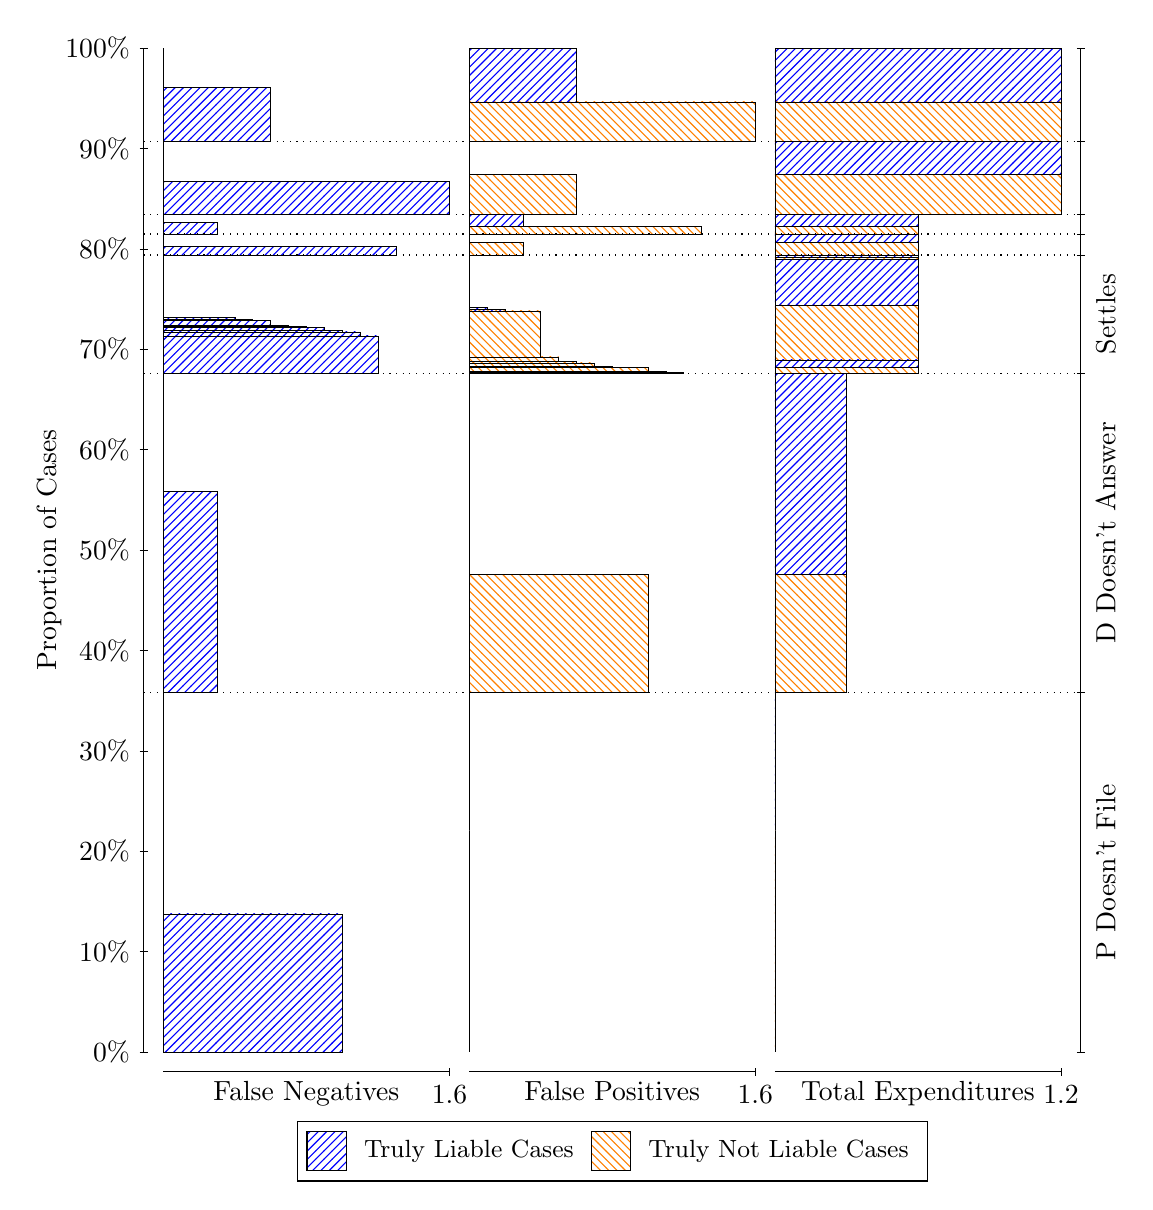
\begin{tikzpicture}
\draw[black, very thin] (1.5,1.75) -- (1.5,14.5);
\node[rotate=90, anchor=center] at (0.3, 8.125) {Proportion of Cases};
\draw[black, very thin] (1.45,1.75) -- (1.55,1.75);
\node[anchor=east] at (1.45, 1.75) {0\%};
\draw[black, very thin] (1.45,3.025) -- (1.55,3.025);
\node[anchor=east] at (1.45, 3.025) {10\%};
\draw[black, very thin] (1.45,4.3) -- (1.55,4.3);
\node[anchor=east] at (1.45, 4.3) {20\%};
\draw[black, very thin] (1.45,5.575) -- (1.55,5.575);
\node[anchor=east] at (1.45, 5.575) {30\%};
\draw[black, very thin] (1.45,6.85) -- (1.55,6.85);
\node[anchor=east] at (1.45, 6.85) {40\%};
\draw[black, very thin] (1.45,8.125) -- (1.55,8.125);
\node[anchor=east] at (1.45, 8.125) {50\%};
\draw[black, very thin] (1.45,9.4) -- (1.55,9.4);
\node[anchor=east] at (1.45, 9.4) {60\%};
\draw[black, very thin] (1.45,10.675) -- (1.55,10.675);
\node[anchor=east] at (1.45, 10.675) {70\%};
\draw[black, very thin] (1.45,11.95) -- (1.55,11.95);
\node[anchor=east] at (1.45, 11.95) {80\%};
\draw[black, very thin] (1.45,13.225) -- (1.55,13.225);
\node[anchor=east] at (1.45, 13.225) {90\%};
\draw[black, very thin] (1.45,14.5) -- (1.55,14.5);
\node[anchor=east] at (1.45, 14.5) {100\%};

\draw[black, very thin] (13.4,1.75) -- (13.4,14.5);
\draw[black, very thin] (13.35,1.75) -- (13.45,1.75);
\node[anchor=west] at (13.35, 1.75) {};
\draw[black, very thin] (13.35,6.3124) -- (13.45,6.3124);
\node[anchor=west] at (13.35, 6.3124) {};
\draw[black, very thin] (13.35,10.371) -- (13.45,10.371);
\node[anchor=west] at (13.35, 10.371) {};
\draw[black, very thin] (13.35,11.872) -- (13.45,11.872);
\node[anchor=west] at (13.35, 11.872) {};
\draw[black, very thin] (13.35,12.138) -- (13.45,12.138);
\node[anchor=west] at (13.35, 12.138) {};
\draw[black, very thin] (13.35,12.386) -- (13.45,12.386);
\node[anchor=west] at (13.35, 12.386) {};
\draw[black, very thin] (13.35,13.316) -- (13.45,13.316);
\node[anchor=west] at (13.35, 13.316) {};
\draw[black, very thin] (13.35,14.5) -- (13.45,14.5);
\node[anchor=west] at (13.35, 14.5) {};

\draw[black, very thin, pattern color=blue, pattern=north east lines] (1.75,1.75) rectangle (4.0208,3.5025);
\draw[black, very thin, pattern color=orange, pattern=north west lines] (1.75,3.5025) rectangle (1.75,6.3124);
\draw[black, very thin, pattern color=blue, pattern=north east lines] (1.75,6.3124) rectangle (2.4312,8.865);
\draw[black, very thin, pattern color=orange, pattern=north west lines] (1.75,8.865) rectangle (1.75,10.371);
\draw[black, very thin, pattern color=blue, pattern=north east lines] (1.75,10.371) rectangle (4.475,10.843);
\draw[black, very thin, pattern color=blue, pattern=north east lines] (1.75,10.843) rectangle (4.2479,10.894);
\draw[black, very thin, pattern color=blue, pattern=north east lines] (1.75,10.894) rectangle (4.0208,10.911);
\draw[black, very thin, pattern color=blue, pattern=north east lines] (1.75,10.911) rectangle (3.7937,10.952);
\draw[black, very thin, pattern color=blue, pattern=north east lines] (1.75,10.952) rectangle (3.7937,10.953);
\draw[black, very thin, pattern color=blue, pattern=north east lines] (1.75,10.953) rectangle (3.5667,10.969);
\draw[black, very thin, pattern color=blue, pattern=north east lines] (1.75,10.969) rectangle (3.3396,10.977);
\draw[black, very thin, pattern color=blue, pattern=north east lines] (1.75,10.977) rectangle (3.1125,11.041);
\draw[black, very thin, pattern color=blue, pattern=north east lines] (1.75,11.041) rectangle (2.8854,11.058);
\draw[black, very thin, pattern color=blue, pattern=north east lines] (1.75,11.058) rectangle (2.6583,11.082);
\draw[black, very thin, pattern color=orange, pattern=north west lines] (1.75,11.082) rectangle (1.75,11.872);
\draw[black, very thin, pattern color=blue, pattern=north east lines] (1.75,11.872) rectangle (4.7021,11.983);
\draw[black, very thin, pattern color=orange, pattern=north west lines] (1.75,11.983) rectangle (1.75,12.138);
\draw[black, very thin, pattern color=blue, pattern=north east lines] (1.75,12.138) rectangle (2.4312,12.285);
\draw[black, very thin, pattern color=orange, pattern=north west lines] (1.75,12.285) rectangle (1.75,12.386);
\draw[black, very thin, pattern color=blue, pattern=north east lines] (1.75,12.386) rectangle (5.3833,12.805);
\draw[black, very thin, pattern color=orange, pattern=north west lines] (1.75,12.805) rectangle (1.75,13.316);
\draw[black, very thin, pattern color=blue, pattern=north east lines] (1.75,13.316) rectangle (3.1125,13.999);
\draw[black, very thin, pattern color=orange, pattern=north west lines] (1.75,13.999) rectangle (1.75,14.5);
\draw[black, very thin, pattern color=orange, pattern=north west lines] (5.6333,1.75) rectangle (5.6333,4.56);
\draw[black, very thin, pattern color=blue, pattern=north east lines] (5.6333,4.56) rectangle (5.6333,6.3124);
\draw[black, very thin, pattern color=orange, pattern=north west lines] (5.6333,6.3124) rectangle (7.9042,7.8186);
\draw[black, very thin, pattern color=blue, pattern=north east lines] (5.6333,7.8186) rectangle (5.6333,10.371);
\draw[black, very thin, pattern color=orange, pattern=north west lines] (5.6333,10.371) rectangle (8.3583,10.385);
\draw[black, very thin, pattern color=orange, pattern=north west lines] (5.6333,10.385) rectangle (8.1313,10.395);
\draw[black, very thin, pattern color=orange, pattern=north west lines] (5.6333,10.395) rectangle (7.9042,10.441);
\draw[black, very thin, pattern color=orange, pattern=north west lines] (5.6333,10.441) rectangle (7.6771,10.447);
\draw[black, very thin, pattern color=orange, pattern=north west lines] (5.6333,10.447) rectangle (7.45,10.461);
\draw[black, very thin, pattern color=orange, pattern=north west lines] (5.6333,10.461) rectangle (7.2229,10.501);
\draw[black, very thin, pattern color=orange, pattern=north west lines] (5.6333,10.501) rectangle (6.9958,10.518);
\draw[black, very thin, pattern color=orange, pattern=north west lines] (5.6333,10.518) rectangle (6.7687,10.578);
\draw[black, very thin, pattern color=orange, pattern=north west lines] (5.6333,10.578) rectangle (6.5417,11.162);
\draw[black, very thin, pattern color=blue, pattern=north east lines] (5.6333,11.162) rectangle (6.0875,11.185);
\draw[black, very thin, pattern color=blue, pattern=north east lines] (5.6333,11.185) rectangle (5.8604,11.203);
\draw[black, very thin, pattern color=blue, pattern=north east lines] (5.6333,11.203) rectangle (5.6333,11.872);
\draw[black, very thin, pattern color=orange, pattern=north west lines] (5.6333,11.872) rectangle (6.3146,12.027);
\draw[black, very thin, pattern color=blue, pattern=north east lines] (5.6333,12.027) rectangle (5.6333,12.138);
\draw[black, very thin, pattern color=orange, pattern=north west lines] (5.6333,12.138) rectangle (8.5854,12.239);
\draw[black, very thin, pattern color=blue, pattern=north east lines] (5.6333,12.239) rectangle (6.3146,12.386);
\draw[black, very thin, pattern color=orange, pattern=north west lines] (5.6333,12.386) rectangle (6.9958,12.897);
\draw[black, very thin, pattern color=blue, pattern=north east lines] (5.6333,12.897) rectangle (5.6333,13.316);
\draw[black, very thin, pattern color=orange, pattern=north west lines] (5.6333,13.316) rectangle (9.2667,13.817);
\draw[black, very thin, pattern color=blue, pattern=north east lines] (5.6333,13.817) rectangle (6.9958,14.5);
\draw[black, very thin, pattern color=orange, pattern=north west lines] (9.5167,1.75) rectangle (9.5167,4.56);
\draw[black, very thin, pattern color=blue, pattern=north east lines] (9.5167,4.56) rectangle (9.5167,6.3124);
\draw[black, very thin, pattern color=orange, pattern=north west lines] (9.5167,6.3124) rectangle (10.425,7.8186);
\draw[black, very thin, pattern color=blue, pattern=north east lines] (9.5167,7.8186) rectangle (10.425,10.371);
\draw[black, very thin, pattern color=orange, pattern=north west lines] (9.5167,10.371) rectangle (11.333,10.442);
\draw[black, very thin, pattern color=blue, pattern=north east lines] (9.5167,10.442) rectangle (11.333,10.539);
\draw[black, very thin, pattern color=orange, pattern=north west lines] (9.5167,10.539) rectangle (11.333,11.238);
\draw[black, very thin, pattern color=blue, pattern=north east lines] (9.5167,11.238) rectangle (11.333,11.819);
\draw[black, very thin, pattern color=orange, pattern=north west lines] (9.5167,11.819) rectangle (11.333,11.839);
\draw[black, very thin, pattern color=blue, pattern=north east lines] (9.5167,11.839) rectangle (11.333,11.872);
\draw[black, very thin, pattern color=orange, pattern=north west lines] (9.5167,11.872) rectangle (11.333,12.027);
\draw[black, very thin, pattern color=blue, pattern=north east lines] (9.5167,12.027) rectangle (11.333,12.138);
\draw[black, very thin, pattern color=orange, pattern=north west lines] (9.5167,12.138) rectangle (11.333,12.239);
\draw[black, very thin, pattern color=blue, pattern=north east lines] (9.5167,12.239) rectangle (11.333,12.386);
\draw[black, very thin, pattern color=orange, pattern=north west lines] (9.5167,12.386) rectangle (13.15,12.897);
\draw[black, very thin, pattern color=blue, pattern=north east lines] (9.5167,12.897) rectangle (13.15,13.316);
\draw[black, very thin, pattern color=orange, pattern=north west lines] (9.5167,13.316) rectangle (13.15,13.817);
\draw[black, very thin, pattern color=blue, pattern=north east lines] (9.5167,13.817) rectangle (13.15,14.5);
\draw[black, dotted] (1.5,6.3124) -- (13.4,6.3124);
\draw[black, dotted] (1.5,10.371) -- (13.4,10.371);
\draw[black, dotted] (1.5,11.872) -- (13.4,11.872);
\draw[black, dotted] (1.5,12.138) -- (13.4,12.138);
\draw[black, dotted] (1.5,12.386) -- (13.4,12.386);
\draw[black, dotted] (1.5,13.316) -- (13.4,13.316);
\draw[black, very thin] (1.75,1.5) -- (5.3833,1.5);
\node[anchor=north] at (3.5667, 1.5) {False Negatives};
\draw[black, very thin] (5.3833,1.45) -- (5.3833,1.55);
\node[anchor=north] at (5.3833, 1.45) {1.6};

\draw[black, very thin] (5.6333,1.5) -- (9.2667,1.5);
\node[anchor=north] at (7.45, 1.5) {False Positives};
\draw[black, very thin] (9.2667,1.45) -- (9.2667,1.55);
\node[anchor=north] at (9.2667, 1.45) {1.6};

\draw[black, very thin] (9.5167,1.5) -- (13.15,1.5);
\node[anchor=north] at (11.333, 1.5) {Total Expenditures};
\draw[black, very thin] (13.15,1.45) -- (13.15,1.55);
\node[anchor=north] at (13.15, 1.45) {1.2};

\node[black, centered, rotate=90] at (13.72, 4.0312) {P Doesn't File};
\node[black, centered, rotate=90] at (13.72, 8.3418) {D Doesn't Answer};
\node[black, centered, rotate=90] at (13.72, 11.122) {Settles};





\draw (7.449999999999999,1.5) node[draw=none] (baseCoordinate) {};
\begin{scope}[align=center]
        \matrix[scale=0.5, draw=black, below=0.5cm of baseCoordinate, nodes={draw}, column sep=0.1cm]{
            \node[rectangle, draw, minimum width=0.5cm, minimum height=0.5cm, pattern=north east lines, pattern color=blue] {}; &
            \node[draw=none, font=\small] (B) {Truly Liable Cases}; &
            \node[rectangle, draw, minimum width=0.5cm, minimum height=0.5cm, pattern=north west lines, pattern color=orange] {}; &
            \node[draw=none, font=\small] (B) {Truly Not Liable Cases}; \\
            };
\end{scope}

\end{tikzpicture}
\end{document}